\section{研究背景及意义}
随着现代科技的飞速发展,数字图像成为了人们获取信息、传达思想的重要载体。而高质量的数字图像可以给人们带来更加真实、清晰的视觉体验,或在监控、救灾等领域起到重要的作用。而实际应用中,由于图像采集设备、传输通道等原因,图像常常受到噪声、模糊、压缩、下采样等各种退化影响,使得其分辨率较低,缺乏细节信息,不利于人类的使用。因此在计算机视觉领域中,图像超分辨率(Single Image Super-resolution, SISR)技术成为了一个备受关注的研究方向。

图像超分辨技术的目的是通过将低分辨率图像提高分辨率,从而得到更加清晰、细节更加丰富的图像。早期的超分辨率技术主要研究合成图像的超分辨率,通常假设高分辨率图像经由高斯模糊与双三次下采样过程退化为低分辨率图像。传统的方法包括插值、稀疏表示等,而借由深度学习技术,研究者已提出许多优秀的合成图像的超分辨率模型。但将这些模型应用于真实图像时,会发现效果严重下降。由于真实图像的退化可能是由多种且未知的因素引起的,图像超分辨率处理难度较大。因此,如何提高真实图像的分辨率成为了图像超分辨技术中的重要研究方向。

在真实图像超分辨率中,基于图像退化模型估计的真实图像超分辨方法因其能够通过模拟图像退化过程来获取更加真实的成对高、低分辨率图像数据集用以训练超分辨率网络,而备受关注。这种方法能够在不同程度的噪声和模糊条件下提供更加清晰、细节更加丰富的超分辨图像。因此,本文将研究基于图像退化模型估计的真实图像超分辨方法,探索一种更加高效、准确的图像超分辨技术。

本文将对图像退化过程进行建模,通过合理的退化过程,生成更加真实且多样性的低分辨率图像,并在实验中进行评估,验证其与真实图像的相似性,进而使得能够通过生成的低分辨率图像训练一个超分辨率网络,使其具有将真实的低分辨率图像重建为高分辨率图像的能力。该研究成果可以为图像超分辨领域的相关研究提供借鉴和参考,同时也可以为图像采集、传输等领域的研究提供更加深刻的思考和理解,有助于推动图像处理技术的发展。另外,随着人工智能技术的不断发展,图像超分辨技术也逐渐应用于各个领域,如摄影、视频监控、医疗影像等。因此,本文的研究也具有重要的实际应用价值。

综上所述,本文将探究基于图像退化模型估计的真实图像超分辨方法,旨在提高真实图像的超分辨率,并为图像处理技术的发展和应用提供借鉴和参考。该研究成果对于推动图像超分辨技术在各个领域的应用和发展具有重要意义。
\section{研究现状}
% \subsection{传统的超分辨率技术}
% 图像超分辨率技术是一项具有悠久历史的技术,由于其广泛的应用场景,许多早期的研究人员已经从传统的图像处理技术或者机器学习技术出发提出了许多方法。早期的方法包括插值、稀疏表示、局部嵌入等,这些方法具有图像重建速度快的优势,但在图像质量上,往往会具有较多的锯齿、伪影,对图像细节的还原能力较差,不能与现今基于神经网络的模型相比。

% \subsection{基于深度学习的超分辨率}
% 随着深度学习技术在计算机视觉领域崭露头角和高算力计算设备的问世,自2014年起,基于深度学习的模型逐渐成为图像超分辨率技术的主流。早期的模型\cite{SRCNN}通过将传统方法中的稀疏编码抽象为卷积操作,从而设计出了基于卷积神经网络的超分辨率模型。使用卷积神经网络后,不仅使得训练过程中模型收敛速度更快,降低训练时间成本,也使得图像在重建精度上显著提升。后续的工作中,研究者们从模型深度、残差连接、密集(dense)连接等角度对基于卷积神经网络的模型进行了改进优化,进一步提升了其超分辨率质量。

% \subsection{真实图像的超分辨率}
% 早期的超分辨率模型往往假设高分辨率图像是通过高斯模糊和双三次下采样退化为低分辨率图像。当将这些模型应用于真实场景下时,会发现超分辨率效果显著下降。这是由于真实高分辨率图像是通过噪声、模糊、图像压缩等未知且复杂的方式退化为低分辨率图像,导致真实的低分辨率图像与合成的低分辨率图像在纹理细节、模糊程度等方面完全不一致。为了解决真实图像超分辨率的问题,一个显而易见解决方式是使用真实成对的数据集进行训练。然而,真实成对的数据集采集过程中往往需要耗费大量的人力物力财力,且一般体量不大。故许多研究人员考虑使用无监督学习技术来训练超分辨率网络。基于无监督学习的超分辨率模型可以分为两种类型:其一利用生成对抗模型\cite{goodfellow2020generative}(GAN),让生成器生成类似于真实高分辨率(清晰)图像的图像,而利用鉴别器判别生成图像和真实高分辨率图像(非成对)的真实性;另一种则从如何获取成对数据集入手,先训练一个降采样网络,用以生成拟真的低分辨率图像,以组成伪成对的数据集,再使用此成对数据集训练一个超分辨率网络。本文基于的工作USR-DU\cite{ijcai2022p176}即为第二种类型,USR-DU模型在此基础上加入了不确定性学习,让模型的退化拥有了不确定性,从而能够生成更合理的低分辨率图像。然而,由于USR-DU的降采样部分没有充分利用真实低分辨率图像的模糊信息,故在较为模糊的图像域上不能生成较为合理的拟真低分辨率图像。

\subsection{合成图像超分辨率技术}
早期,许多超分辨率模型通常假设高分辨率图像是通过高斯模糊和双三次下采样退化为低分辨率图像的,其训练集与测试集都是采用上述退化过程产生的合成数据集。我们称这些方法为合成图像的超分辨率技术。
\subsubsection*{传统的图像超分辨率技术}
在2014年以前,图像超分辨率技术主要采用计算机视觉领域中传统的方法。其中包括插值、稀疏表示、局部嵌入等,其中最基础的方法是基于插值算法的上采样。常用的插值算法可分为双线性插值、双二次插值和双三次插值,其精细度依次增加,其中,双三次插值会根据周围16个像素计算目标像素值。由于超分辨率是使图像的像素增加的过程,这意味着原图中的像素之间将会加入更多像素。由于图像的像素是离散的,而我们并不知道真实的描述图像的连续函数$f(x,y)$,故为了确定新增像素的值,可以使用插值算法,即给出一个插值函数$g(x,y)$,其中对于图像中的每个像素$f(x_i,y_i)$,有$g(x_i,y_i)=f(x_i,y_i)$。对于新增的像素点,使用插值函数算出其值即可。插值算法的优点是简单、快速,缺点是不够真实,不能补充较为详细的细节信息。

随着技术的发展,稀疏表示方法逐渐成为研究的热点。Yang等人\cite{4587647}指出,可将图像分解为字典$D$与原子$\alpha$,其中高、低分辨率图像的原子类似,而字典不同。此算法首先使用成对的高低分辨率数据集训练字典,在推理时,通过字典$D_l$计算出低分辨率图像的原子,再使用此原子与高分辨率图像的字典$D_h$计算出高分辨率图像。由于最初的稀疏表示方法没有考虑图像的噪声、模糊的问题,Dong等人\cite{6392274}提出了稀疏编码噪声的概念,将算法优化目标转为降低稀疏编码噪声,通过图像非局部自相似性获得了对图像稀疏编码的良好估计。稀疏编码方法在PSNR与SSIM\cite{wang2002universal}指标上较插值算法更高,也能还原更多的细节,但生成的高分辨率图像中带有较为明显的锯齿。


\subsubsection*{基于卷积神经网络的超分辨率技术}
随着AlexNet\cite{NIPS2012_c399862d}在2012年的ImageNet竞赛中得冠,基于深度卷积神经网络的模型逐渐进入计算机视觉研究者的视野,而后续的VGG\cite{simonyan2014very}、GoogleNet\cite{szegedy2015going}等则更让此类方法成为了计算机视觉研究的主流。2014年,Dong等人\cite{SRCNN}提出了基于卷积神经网络的SRCNN,开创了使用深度学习方法研究图像超分辨率问题的先河。作者将传统稀疏表示方法的过程抽象为三层卷积神经网络,其中第一层提取低分辨率图像的特征图,第二层将特征图与高分辨率图像的稀疏表示相对应,第三层结合空间邻域的预测完成高分辨率图像的重建。SRCNN在保证其推理速度更快的同时,其超分辨率效果远超其他传统模型。

由于SRCNN只有三层,其并没有完全利用深度卷积神经网络的优势。在接下来一段时间中,研究者提出了多种改进模型,从模型深度\cite{vedaldi15matconvnet}、残差连接\cite{Lim_2017_CVPR_Workshops}、密集(dense)连接\cite{wang2018esrgan}等角度对基于卷积神经网络的超分辨率模型进行了优化,使模型在准确度方面有了进一步的提升。但对于较大的放大倍数,这些模型却无法恢复出较为精细的纹理细节。随着生成对抗网络\cite{goodfellow2020generative}(GAN)这一框架在计算机视觉领域中逐渐流行,Ledig等人\cite{fritsche2019frequency}提出了基于GAN的模型SRGAN,对大的放大倍率来说,可以重建出更为真实的高分辨率图像。此后,超分辨率模型多会基于GAN设计,本文亦是如此。



\subsection{真实图像超分辨率技术}
早期的超分辨率模型往往假设高分辨率图像是通过高斯模糊和双三次下采样退化为低分辨率图像。当将这些模型应用于真实场景下时,会发现超分辨率效果显著下降。这是由于真实高分辨率图像是通过噪声、模糊、图像压缩等未知且复杂的方式退化为低分辨率图像,导致真实的低分辨率图像与合成的低分辨率图像在纹理细节、模糊程度等方面完全不一致,故以往的合成图像超分辨率模型并不能很好地迁移到真实场景下。

为了解决真实图像的超分辨率问题,可以使用真实成对的数据集(如City100\cite{chen2019camera},RealSR\cite{cai2019toward}等)训练超分辨率网络,从而提升模型对真实图像的重建能力。但是,从一方面来说,真实成对数据集的采集工作是费时费力且高成本的,故无法取得大量的;从另一方面来说,对于某些任务来说(如修复老照片,老电影等),低分辨率图像本身没有对应的高分辨率图像,无法进行监督式的训练。因此,必须对模型本身进行改进,以满足真实图像超分辨率任务的需求。在发展早期阶段,Yuan等人\cite{yuan2018unsupervised}提出了无监督模型CinCGAN,如图\ref{fig:CinCGAN}。作者利用两个CycleGAN\cite{zhu2017unpaired},分别将低分辨率图像进行去模糊去噪处理和超分辨率,其中生成性损失通过重构损失和内容损失(identity loss)计算,第一个网络使用干净的非成对的低分辨率图像$y$计算对抗性损失,而第二个网络使用非成对的高分辨率图像$z$计算对抗性损失。为了增强GAN的输入和输出之间的一致性,即确保生成的干净低分辨率图像和高分辨率图像是基于输入的低分辨率图像的,作者用两个额外的生成器生成了$x'$和$x''$计算循环一致性损失。作为无监督模型,CinCGAN取得了和监督式模型相当的超分辨率效果,但由于模型结构过于复杂,带来了训练、推理速度上的下降。

\begin{figure}[htbp]
    \centering
    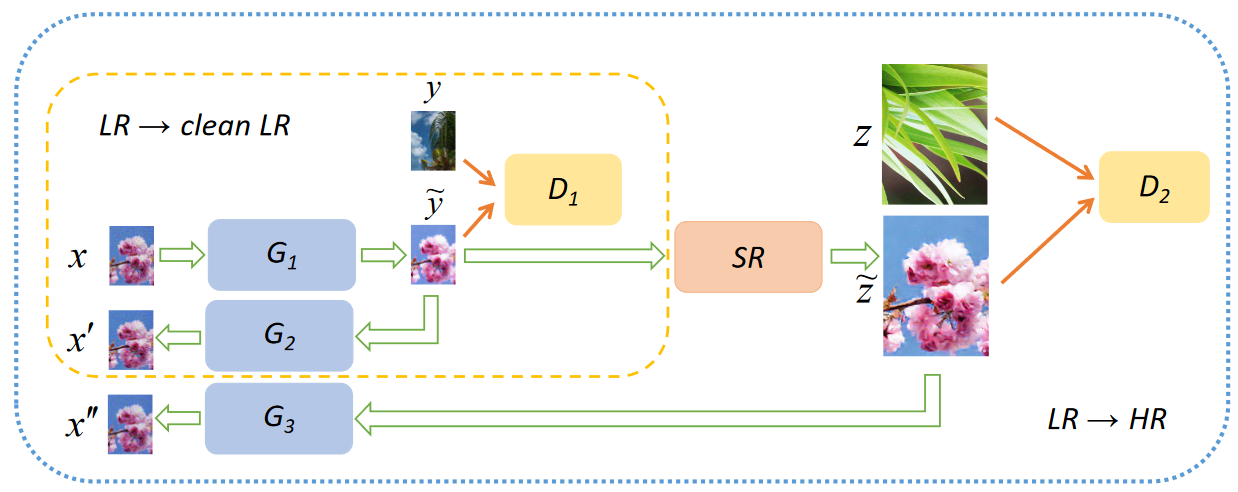
\includegraphics[width=1.0\textwidth]{imgs/CinCGAN.png}
    \caption{CinCGAN}
    \label{fig:CinCGAN}
\end{figure}

为了能以较小的计算成本去训练一个更具泛化性的模型,Fritsche等人\cite{fritsche2019frequency}开创性地提出了DSGAN模型,意为DownSampleGAN。该模型由两部分组成,依次进行训练。其中,第一部分为下采样模型,将高分辨率图像退化为贴近真实的低分辨率图像,其流程如图\ref{fig:DSGAN-DSN},即先对高分辨率图像双三次下采样,再生成拟真的低分辨率图像。而第二部分为超分辨率模型,如图\ref{fig:DSGAN-SRN},使用第一部分模型生成的伪成对数据集进行训练。通过此方式,超分辨率模型可以轻松地在大量成对数据集上进行训练,有效提高了模型的超分效果和稳定性。在这一模型框架的基础上,许多后续工作在生成图像与真实图像的域差距\cite{Wei_2021_CVPR}、显式估计模糊核\cite{fang2022uncertainty}\cite{liang2021mutual}\cite{fangself}、退化的随机性\cite{wang2021realesrgan}等方面优化了其的性能泛化性。

\begin{figure}[htbp]
    \subcaptionbox{\label{fig:DSGAN-DSN}}{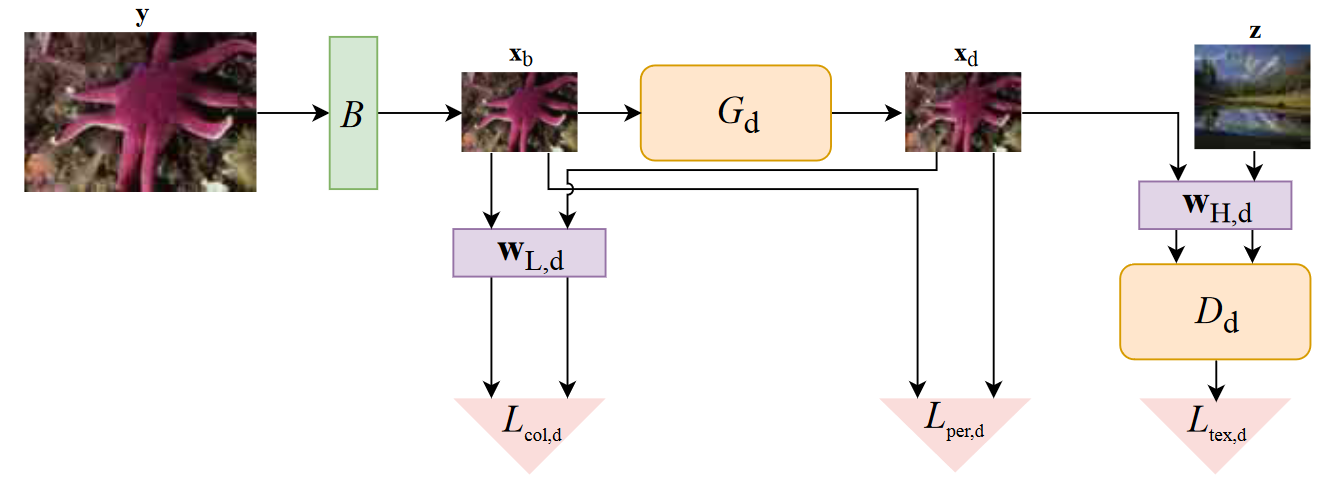
\includegraphics[width=.5\linewidth]{imgs/DSGAN_DSN.png}}\hfill
    \subcaptionbox{\label{fig:DSGAN-SRN}}{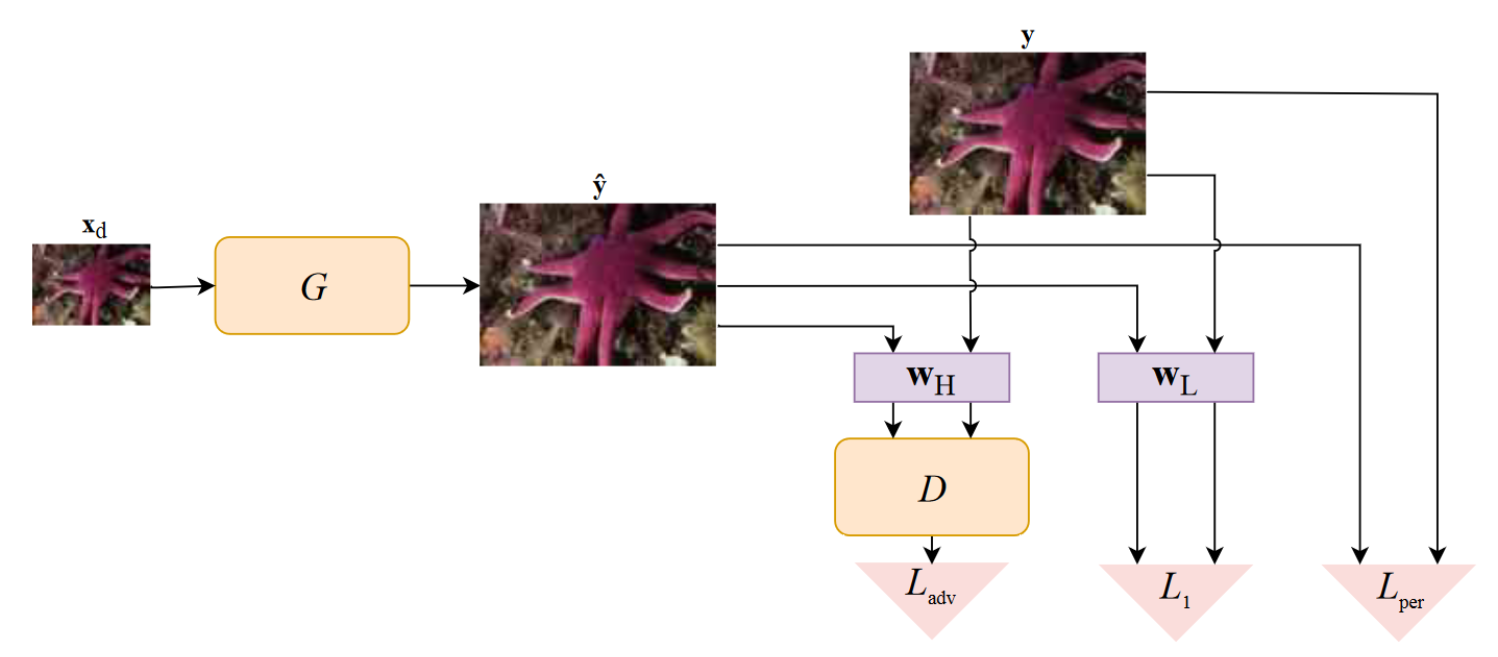
\includegraphics[width=.5\linewidth]{imgs/DSGAN_SRN.png}}
    \caption{DSGAN的结构:其中,图(a)为降采样网络(DSN),图(b)为超分辨率网络(SRN)}	
    \label{fig:DSGAN}
\end{figure}

尽管上述方法可以很方便地大量生成伪成对数据集,其生成的图像与真实世界中退化产生的图像仍有一定差距,这是由于从理论上来说,这些模型假定图像的退化过程是确定性的,即一张高分辨率图像只能退化为一张低分辨率图像。而实际情景中,由于各种因素影响,图像的退化过程往往是具有不确定性的,即一张高分辨率图像可以经由不同的方式退化为不同的低分辨率图像。为了估计这种不确定性,并将其用于更好地生成低分辨率图像,Ning等人\cite{ijcai2022p176}提出基于不确定性学习的无监督超分辨率模型USR-DU,模型的整体结构如图\ref{fig:USR-DU}所示。在模型的降采样部分中,同时学习了低分辨率图像的生成及其不确定性,基于以二者为参数的拉普拉斯分布采样,可以采得多幅不同但相似的低分辨率图像,可以作为超分网络的训练集使用。模型在多个数据集上的表现超过了当前最先进的模型,但是,当将此模型应用到模型性较大的数据集(如RealSR)中时,其超分辨率性能有所下降。这是由于其DSN部分未能充分利用真实低分辨率图像中的模糊信息,直接使用了干净的双三次下采样图像作为内容和感知损失函数中的参考图像,而如何在DSN中引入模糊信息,则是本文研究的重点。



\begin{figure}[htbp]
    \centering
    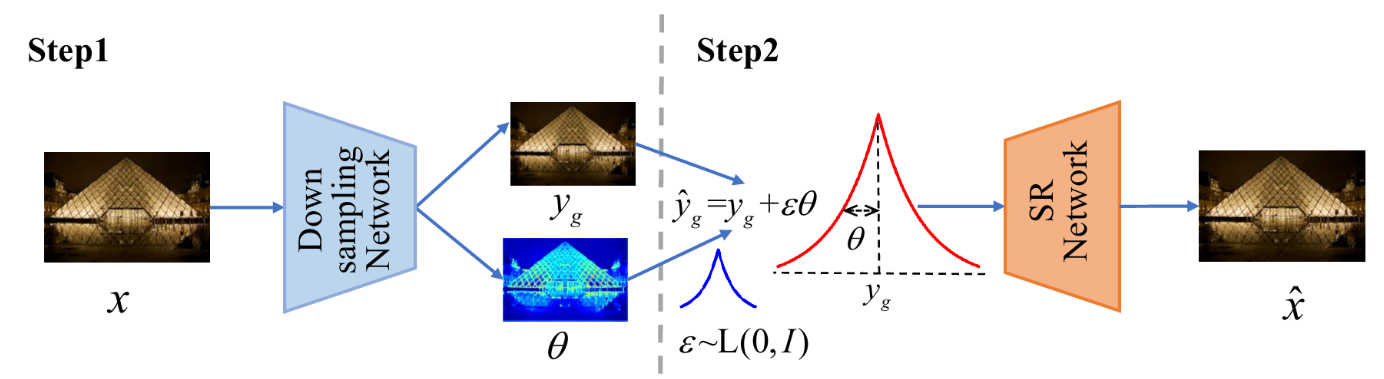
\includegraphics[width=1.0\textwidth]{imgs/USR-DU.png}
    \caption{USR-DU}
    \label{fig:USR-DU}
\end{figure}




\subsection{基于模糊核估计的盲图像超分辨率技术}
除了上述方法,也有部分工作采取显式估计模糊核,并将模糊核作为特征融合到超分辨率网络中的方式来训练真实图像超分辨率模型。其中,Liang等人\cite{liang2021mutual}提出了MANet,训练了一个空间变化地估计低分辨率图像模糊核的网络,该网络针对给定低分辨率图像,会估计其对应高分辨率图像在退化过程中每个像素点所采用的模糊核,图\ref{fig:KE_SV}中给出了一个例子:图中各处均拥有不同的模糊核。作者将估计出的模糊核作为特征融合到修改过的RRDB-SFT超分网络中,对其进行微调,从而实现真实图像超分辨率。Fang等人\cite{fang2022uncertainty}提出了KULNet,同步训练了核估计网络和超分辨率网络,并引入了不确定性学习,增强了模型的稳定性。Fang等人\cite{fangself}提出了UFPNet,基于流模型空间可变地估计了运动模糊核,具体来说,首先训练了一个可生成运动模糊核的流模型,再训练了一个模糊核隐代码估计网络,使用估计的隐代码来生成最终的模糊核,其中,隐代码的估计采用了不确定性学习。随后,将估计的模糊核融合到超分辨率网络中。此模型兼顾了\cite{liang2021mutual}\cite{fang2022uncertainty}中空间可变模糊核估计和不确定性学习这两个优势,使得模型的稳定性和准确性进一步增强。本文中,为了解决如何在USR-DU的降采样部分中引入模糊信息的问题,对上述核估计模型的利用必不可少。

% \begin{figure}[h]
%     \centering
%     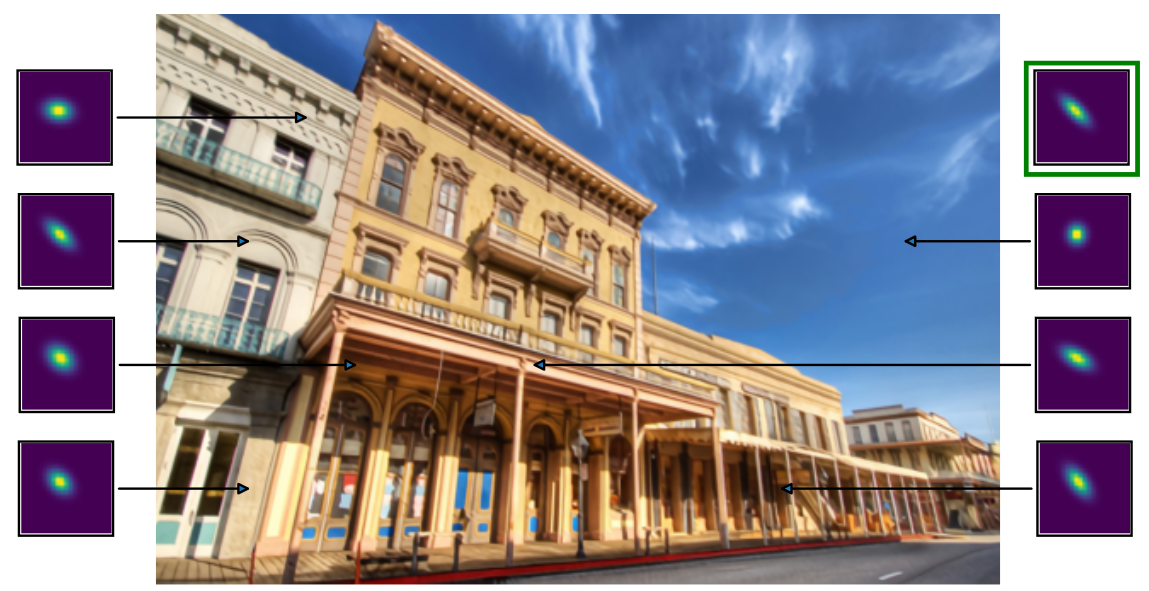
\includegraphics[width=0.5\textwidth]{imgs/KE_SV.png}
%     \caption{空间可变的模糊核估计}
%     \label{fig:KE_SV}
% \end{figure}

\begin{figure}[htbp]
    \centering
    \captionbox{USR-DU的降采样网络\label{fig:USR-DU-DSN}}{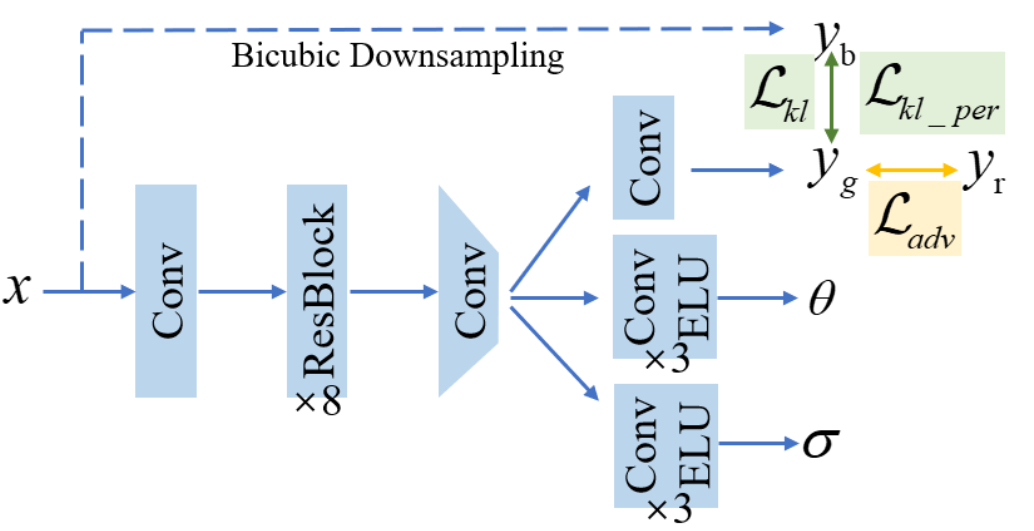
\includegraphics[width=.5\linewidth]{imgs/USR-DU-DSN.png}}\hfill
    \captionbox{空间可变的模糊核估计\label{fig:KE_SV}}{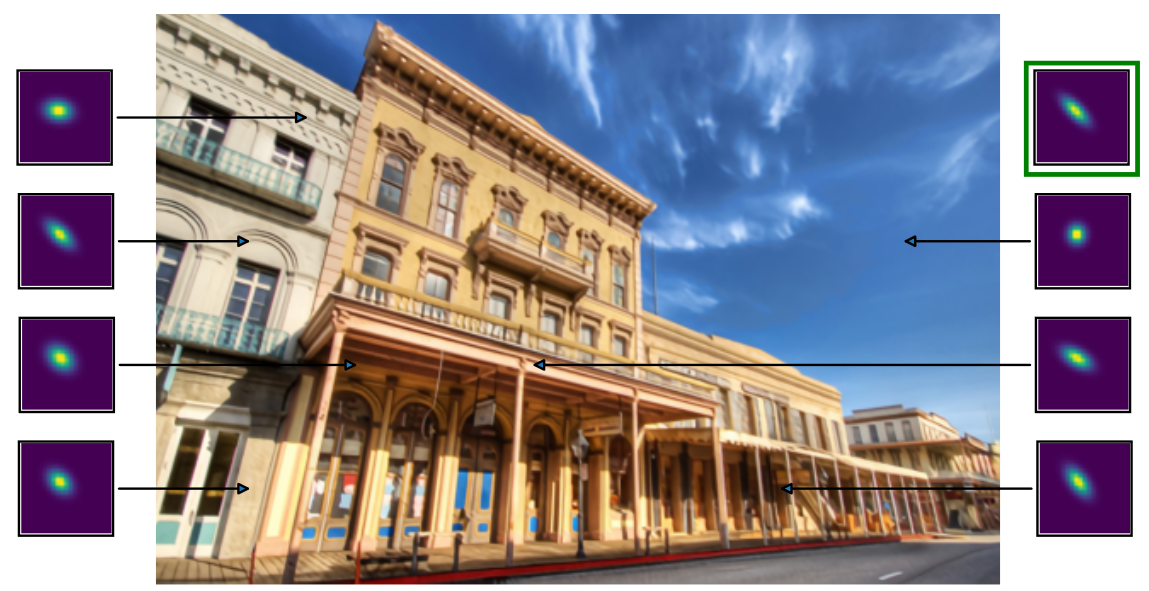
\includegraphics[width=.5\linewidth]{imgs/KE_SV.png}}
\end{figure} 



\section{论文的主要内容及工作安排}
本论文主要目的是解决USR-DU模型在模糊信息的利用上不足导致对较模糊的低分辨率图像重建能力较差的问题。为此提出了若干条改进方案,形成了改进模型UBSR-DU。

第一章阐述了基于退化模型估计的真实图像超分辨这一研究目标的意义,介绍了有关图像超分辨率这一领域的发展历史和相关工作。

第二章介绍了超分辨率任务评价指标、超分辨率模型相关工作、图像模糊核估计方法、超分辨率任务数据集等本文所使用的相关技术。

第三章分析了USR-DU具有什么样的缺陷,并指出这种缺陷来自于模型的DSN部分对真实低分辨率图像模糊信息的忽略。进而提出了引入真实图像模糊信息的可选方案,通过实验得出了最佳改进方案。随后,经过详细的消融实验验证了此方案的有效性、可靠性和必要性。最后,比较了提出的模型与现有最先进的模型之间的效果、性能差异。

第四章对全文工作进行了总结,给出了所提出模型的局限性,并给出了可行的进一步研究方向。